\documentclass[a4paper]{article}
\usepackage[utf8]{inputenc}


\usepackage{geometry}

\usepackage[mathcal]{euscript}

\usepackage{amsmath, amsfonts, amssymb, amsthm}
\usepackage{mathptmx}
\usepackage{algorithm2e}

\usepackage{graphicx, url}

\usepackage[english, russian]{babel}
\newcommand{\eng}[1]{\foreignlanguage{english}{#1}}
\newcommand{\rus}[1]{\foreignlanguage{russian}{#1}}

\title{Preparation for the finals}
\author{Nazarov Ivan, \rus{101мНОД(ИССА)}\\the DataScience Collective}

\begin{document}
\maketitle

\selectlanguage{english}

\section{\rus{Общие вопросы программы}} % (fold)
\label{sec:general_questions}
\noindent\textbf{Q:}\rus{Классический и ранговый критерии для проверки гипотезы об
однородности двух выборок против альтернативы сдвига.}

\hfill\\\noindent\textbf{A:}

\hfill\\\noindent\textbf{Q:}\rus{Классический и ранговый критерии для проверки гипотезы
об однородности двух выборок против альтернативы масштаба.}

\hfill\\\noindent\textbf{A:}

\hfill\\\noindent\textbf{Q:}\rus{Постановка задачи однофакторного дисперсионного
анализа. Оценивание контрастов в модели однофакторного дисперсионного анализа.}

\hfill\\\noindent\textbf{A:}

\hfill\\\noindent\textbf{Q:}\rus{Применение непараметрических методов в задаче однофакторного
дисперсионного анализа.}

\hfill\\\noindent\textbf{A:}

\hfill\\\noindent\textbf{Q:}\rus{Кластеризация. Основные методы кластеризации.
Типы исходных данных. Визуализация кластеров.}

\hfill\\\noindent\textbf{A:}

\hfill\\\noindent\textbf{Q:}\rus{Кластеризация методом K-средних. Основные алгоритмы.
Инициализация. Аномальные кластеры.}

\hfill\\\noindent\textbf{A:}

\hfill\\\noindent\textbf{Q:}\rus{Иерархическая кластеризация. Агломеративные и
дивизионные методы.}

\hfill\\\noindent\textbf{A:}

% section general_questions (end)


\section{\rus{Упорядоченные множества в анализе данных}} % (fold)
\label{sec:ordered_sets}

\noindent\textbf{Q:}\rus{Свойства бинарных отношений. Отношения частичного
порядка, эквивалентности, толерантности. Отношения строгого порядка и
покрытия, связанные с отношением частичного порядка. Графы отношений,
диаграммы частичного порядка. Полурешетки, решетки. Два определения решеток
и теорема об их эквивалентности.}

\hfill\\\noindent\textbf{A:}
A binary relation on $\Omega$ is a subset $R\subseteq \Omega\times \Omega$.
The following properties:
\begin{description}
    \item[Reflexivity:] $(x, x)\in R$ for all $x\in\Omega$;
    \item[Anti-reflexivity:] $(x, x)\notin R$ for all $x\in\Omega$;
    \item[Symmetry:] $(x, y)\in R$ implies $(y, x)\in R$;
    \item[Asymmetry:] $(x, y)\in R$ implies $(y, x)\notin R$;
    \item[Anti-symmetry:] $(x, y), (y,x)\in R$ implies $y=x$;
    \item[Transitivity:] $(x,y), (y,z)\in R$ imply $(x,z)\in R$;
    \item[Totality (Completeness):] $\forall x, y\in \Omega$ either $(x,y)\in R$,
    or $(y,x)\in R$, or both.
\end{description}
Binary Relations are equivalent to graphs: if $R$ is a binary relation on $\Omega$
then its graph is $G = (V, E)$ for $V$ -- the set of all elements of $\Omega$
participating in $R$.

\noindent Relation composition: for two binary relations $R_1$ and $R_2$ on $\Omega$
$$ R_1\circ R_2
    = \{(x,z)\in \Omega\times\Omega
        \,:\, \exists y\in \Omega\, (x,y)\in R_1, (y,z)\in R_2\}
    \,. $$
\noindent Transitive closure:
$R^T = \bigcap_{L\in [R]} L$, for $[R]$ -- the set of all transitive binary
relations on $\Omega$ that cover $R$. In fact $R^T = \bigcup_{n\geq1} R^n$,
where $R^n = R\circ \ldots \circ R$ -- $n$ times. Indeed, suppose $R\subseteq M$
for some transitive rlation $M$, then for $(a,b)\in R^T$ there is $n\geq 1$
such that $(a,b)\in R^n$, whence $\exists (u_i)_{i=0}^n\in R$ with $(u_{i-1}, u_i)\in R$
such that $u_0=a$ and $u_n=b$. Since $R\subseteq M$, $(a,b)\in M$ by transitivity.

\noindent Examples: \begin{description}
    \item[Equivalence:] a reflexive, symmetric and transitive relation.
    \item[Tolerance:] a reflexive, symmetric relation.
    ``Equal within threshold'': $\{(a,b)\in \mathbb{R}\,:\, |a-b|\leq \epsilon\}$
    (``likeness'', ``similarity'').
    \item[Quasi-order (preorder):] reflexive and transitive relation.
    ``being isomorphic to a subgraph'': graph isomorphism, $G_1 \sim G_2$, is when
    there is a bijection $\phi:V_1\mapsto V_2$ with $(\phi(u),\phi(v))\in E_2$ iff
    $(u,v)\in E_1)$.
    \item[Partial order:] a reflexive, anti-symmetric, transitive relation.
    $(\mathbb{N}, \leq)$ on natural numbers is total, $(\mathcal{P}(\Omega),
    \subseteq)$ -- partial.
    \item[Strict order:] $(P, \leq)$ -- poset. A strict order is $(P, <)$ such
    that $a<b$ iff $a\leq b$ and $a\neq b$. Strict orders are anti-reflexive,
    asymmetric and transitive.
    \item[Covering relation:] $(P, \leq)$ -- poset. A covering relation is $(P, \prec)$
    such that $a\prec b$ iff $a\leq b$, $a\neq b$ and there is no $z\in P$ with $z\neq a,b$
    and such that $a\leq z\leq b$. Gives rise to Hasse diagrams (fig.~\ref{fig:hasse})
    of partial orders, which are used extensively in FCA.
\end{description}
\begin{figure}
    \centering
    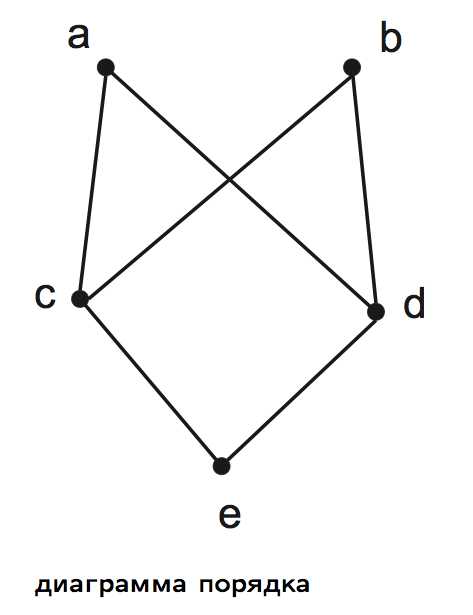
\includegraphics[width=0.35\textwidth]{hasse.png}
    \label{fig:hasse}
    \caption{a hasse diagram.}
\end{figure}

Algebraically a semi-lattice is pair $(L, \diamond)$ such that $\diamond: L\times L \to L$
is idempotent ($a\diamond a=a$), commutative ($a \diamond b = b \diamond a$) and associative
($a \diamond (b \diamond c) = (a \diamond b) \diamond c$). Natural partial order $a\leq b$
iff $a\diamond b = a$ (join).

From the order-theoretic approach, a join semi-lattice is a poset $(L, \leq)$ such
that the supremum (the least upper bound) $\sup\{x, y\}$ exists and unique for every
pair of $x, y \in L$. Similarly, a meet semi-lattice is a poset with a well-defined
pairwise infimum operation (uniqueness). These definitions are equivalent. (see.
\textbf{p.~5} of the notes).

A lattice $(L, \wedge, \vee)$ imposes an extra restriction on the operators:
$$ x = x \wedge (x\vee y) = x \vee ( x\wedge y) \,, $$
called ``absorption''. Note that $(L, \wedge)$ is a join semi-lattice and $(L, \vee)$
is a meet semi-lattice. The natural order on $(L, \wedge, \vee)$ is defined as
$a\leq b$ iff $a\wedge b=a$ (or $a\vee b = b$). A lattice $(L, \wedge, \vee)$ is
modular iff
$$ x\leq z \Rightarrow x \vee (y\wedge z) = (x \vee y ) \wedge z\, \forall y\,. $$

A lattice is distributive iff its Hasse diagram has neither diamonds, nor pentagons.
A lattice is modular iff its Hasse diagram contains no pentagons (fig.~\ref{fig:lattice_pen_di}).
\begin{figure}
    \centering
    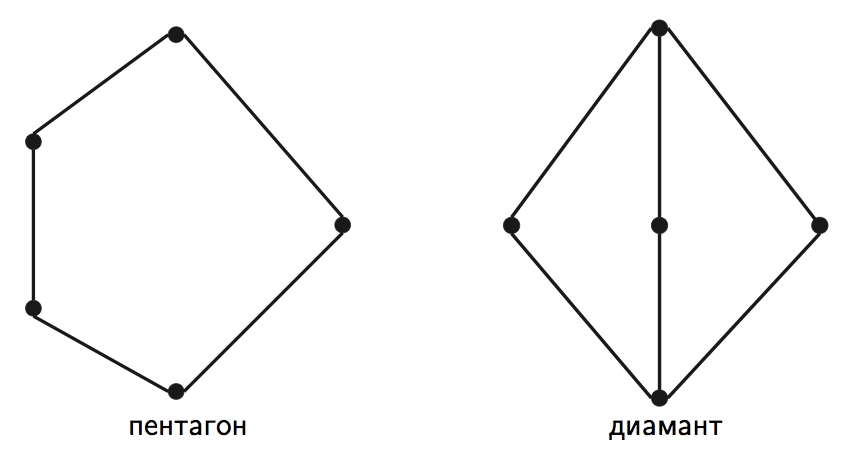
\includegraphics[width=0.35\textwidth]{pents_and_diamonds.png}
    \label{fig:lattice_pen_di}
    \caption{Pentagrams and diamonds.}
\end{figure}

\hfill\\\noindent\textbf{Q:}\rus{Соответствие Галуа, задаваемое бинарным отношением. Оператор
замыкания. Решетки формальных понятий, основная теорема анализа формальных понятий
(АФП): представимость полных решеток решетками понятий. Диаграмма решетки понятий
(граф отношения покрытия).}

\hfill\\\noindent\textbf{A:}
For the Galois connection see \textbf{p.~8}, for closure operator note that it is
defined as the composition of maps of the Galois connection see.~8-9. In general
a closure  operator (not the topological closure) has the following properties:
$[\cdot]: (P, \leq) \mapsto (P, \leq))$ is a closure operator if it is idempotent
($[[a]]=[a]$), extensive ($a\leq [a]$), and monotonic ($[a]\leq [b]$ whenever
$a\leq b$).

\noindent For concept lattices see \textbf{p.~10} and the complete lattice equivalence
see \textbf{p.~11-13}.

\hfill\\\textbf{Q:}\rus{Признаковые импликации в контексте. Базис импликаций Дюкена-
Гига (на основе псевдосодержаний) и генераторный базис. Импликации в контексте и
функциональные зависимости в теории реляционных баз данных (двусторонняя сводимость).}

\hfill\\\textbf{A:}
To summarize, in implication on a context $(G, M, I)$ is a pair $A, B\subseteq M$,
denoted by $A\to B$, if $A'\subseteq B'$ (or $B\subseteq  A$), i.e. all objects that
have all attributes from $A$ also have every attribute from $B$: for all $g\in G$
$$ A\subseteq g' \Rightarrow B \subseteq g'\,, $$
for such $A, B$. For details on implications, and Armstrong rules refer to \textbf{p.~15-19}
of the notes. Implication bases are covered in \textbf{p.~19-21} of the notes.

Based on lecture slides (lecture 5 slides 3-5). A multivalued context is $4$-tuple
$(G, M, W, I)$ with $W$ being the feature value set, $I\subseteq G\times M \times W$
is such that $(g,m,w), (g,m,v)\in I$ implies $w=v$ ($I$ is a map $G\times M\mapsto W$).
An attribute $m$ is complete if for any $g \in G$ there exists $w\in W$ with $(g,m,w)
\in I$. A multivalued context id complete if all its features are complete.
Each feature $m\in M$ in such context can be identified with a map $\phi_m:G\mapsto W$
(shorthand $m(\cdot) = \phi_m(\cdot)$) with $(g, m, m(g))\in I$ for all $m\in M$
and $g\in G$.

A functional dependence $X\mapsto Y$, $X, Y\subseteq M$ in a complete multivalued
context $(G, M, W, I)$ takes place if for each pair $g, h\in G$
$$ (m(g) = m(h)\,,\, \forall m\in X)
    \Rightarrow (n(g) = n(h)\,,\, \forall n\in Y)
    \,. $$

Each complete multivalued context $K = (G, M, W, I)$ it is possible to define a context
$K_N = (\mathcal{P}_2(G), M, I_N)$, where $\mathcal{P}_2(G)$ is the set of all unordered
pairs of distinct elements of $G$ and $I_N$ is given by
$$ (\{g, h\}, m) \in I_N
    \Leftrightarrow m(g) = m(h)
    \,. $$
The a multivalued context $K$ has a functional dependence $X\mapsto Y$ iff the induced
context $K_N$ has an implication $X\to Y$.

For a context $K=(G, M, I)$ it is possible to construct a multivalued context
$K_W$ such that the implication $X\to Y$ takes place in $K$ iff $K_W$ has a functional
dependence $X\mapsto Y$. For example, fig.~\ref{fig:multivalued}:
\begin{figure}
    \centering
    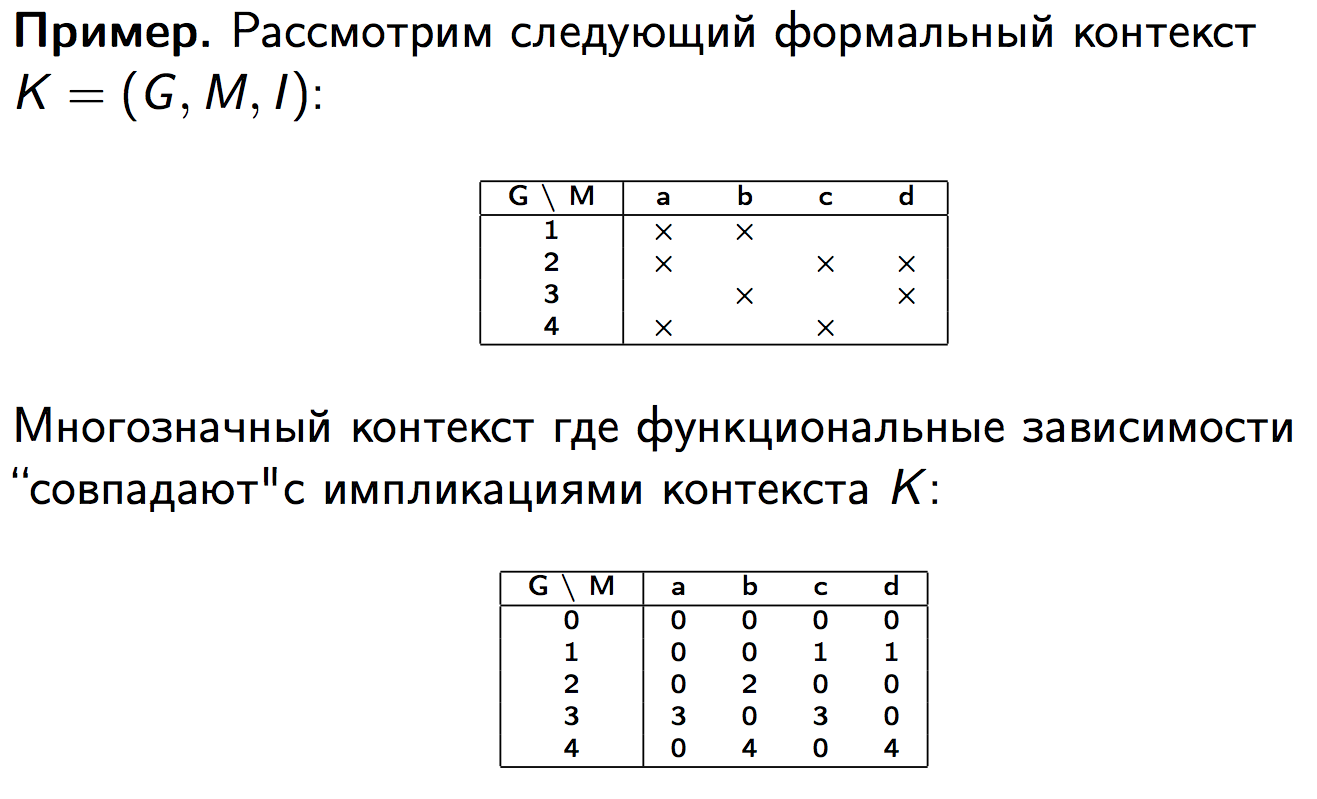
\includegraphics[width=0.5\textwidth]{multivalued.png}
    \label{fig:multivalued}
    \caption{A context and a multivalued context.}
\end{figure}
For further details on the multivalued contexts see \textbf{p.~24-25} of the notes.

\hfill\\\textbf{Q:}\rus{Ассоциативные правила как метод майнинга данных. Поддержка
и достоверность ассоциативных правил. Базис ассоциативных правил и его связь с диаграммой
решетки понятий.}

\hfill\\\textbf{A:}
For implications, support and confidence refer to \textbf{p.~21-22} of the notes.

The ``lift'' of an association rule $A\to B$ is defined as 
$$ \mathtt{lift}(A\to B)
    = \frac{\mathtt{supp}(A\cup B)}{\mathtt{supp}(A)\cdot \mathtt{supp}(B)}
    \,, $$
and measures the departure from independence, The close the ``lift'' is to $1$,
the more likely that there is no underlying connection between $A$ and $B$. Interesting
cases are when the lift is greater than $1$. 

``Apriori'' algorithm (alg.~\ref{alg:apriori}) finds all the association rules in a
context $(G, M, I)$ that have at least the specified level of support ($\frac{|(A\cup B)'|}{|G|}$),
and confidence ($\frac{|(A\cup B)'|}{|A'|}$). The main insight of the algorithm
is that if itemsets (of $M$) are related $A\subseteq B$ then $B'\subseteq A'$ --
the subsets are more frequent, while the supersets are less frequent. This limits
the exponentially large search space.

% \begin{algorithm}
%     \caption{Aprirori algorithm for frequent itemset mining.}\label{alg:apriori}
%     \SetKwInOut{Input}{input}\SetKwInOut{Output}{output}
%     % A poset $(P, \leq)$, and a closure operator $[\cdot]: (P, \leq)\mapsto (P, \leq)$.
%     \Input{A formal context $K$, minimal frequency $\epsilon$.}
%     \Output{A frequent itemsets.}
%     \BlankLine
%     $L_1 \leftarrow \{m\in M\,:\, \mathtt{supp}(m) \geq \epsilon \}$\;
%     $k\leftarrow 2$\;
%     \While{$L_{k-1}\neq \emptyset$}{
%         $C_k \leftarrow \{a \cup \{b\} \,:\, a\in L_{k-1}
%                           \,,\,b\notin a \,,\, b\in M\}$\;
%     }
%     \For{$g \in G \setminus A$}{
%         $(P, Q) \leftarrow \bigl((A \cup \{g\})'', (A \cup \{g\})'\bigr)$\;
%         \tcc{Note that $B \cap \{g\}' = (A\cup \{g\})'$}
%         \If{$\min\{P\setminus A\} \geq g$}{
%         \tcc{or, equivalently, $(P\setminus A) \cap g^\leq$ is empty}
%             $\mathtt{successors} \leftarrow \mathtt{CbO}((P, Q); K)$\;
%             \tcc{these are the immediate successors to $(A, B)$}
%             $\mathtt{concepts} \leftarrow \mathtt{concepts}
%                                           \cup \mathtt{successors}$\;
%         }
%     }
%     Return $\mathtt{concepts}$\;
% \end{algorithm}


\hfill\\\textbf{Q:}\rus{ДСМ-метод в терминах решеток понятий: гипотезы и классификация.
Соотношение ДСМ-гипотез и импликаций. Алгоритмы построения множества всех понятий (полный
перебор и ``Замыкай по одному'').}

\hfill\\\textbf{A:}
\noindent For the JSM method see the \textbf{p.~22-23} of the notes.

\noindent Consider a formal context $K=(G, M, I)$ with a complete order
$(G, \leq)$. Recall that a formal concept is a pair $(A, B)$ such that $A'=B$ and
$B'=A$. Then such pairs are naturally partially ordered by set inclusion (due to
anti-monotonicity of the Galois operators). Put $(A, B) \preceq (P, Q)$ iff $A\subset P$.
The key insight of CbO is that it in order to avoid exhaustive search, the virtual
concept lattice should be traversed in depth-first manner and in special order. In
particular the formal concepts are generated in lexicographic order (a canonical
generation), so that when a closure yields an out-of-order concept, the sub-lattice
of this concept is no longer traversed, because this exact concept has already been
generated by some other closure. The extent-based CbO algorithm is presented in
alg.~\ref{alg:cbo}, where $g^\leq = \{h\in G\,:\,h\leq g\}$ for any $g\in (G, \leq)$.
The full set of formal concepts is given by
$$ \mathtt{concepts}
    \leftarrow \mathtt{CbO}\bigl((\emptyset'', \emptyset'); K\bigr)
    \,. $$
For an intent based CbO, just reverse the roles (polarity) of $G$ and $M$ in the
description and the algorithm. This is due to the duality of the concept lattices.
\begin{algorithm}
    \caption{Intent based Close by One algorithm for $K$.}\label{alg:cbo}
    \SetKwInOut{Input}{input}\SetKwInOut{Output}{output}
    % A poset $(P, \leq)$, and a closure operator $[\cdot]: (P, \leq)\mapsto (P, \leq)$.
    \Input{A formal context $K$, a formal concept $(A, B)$.}
    \Output{A list of immediate descendant formal concepts $(P, Q)$ with $(A, B) \prec
    (P, Q)$.}
    \BlankLine
    $\mathtt{concepts} \leftarrow \{(A, B)\}$\;
    \For{$g \in G \setminus A$}{
        $(P, Q) \leftarrow \bigl((A \cup \{g\})'', (A \cup \{g\})'\bigr)$\;
        \tcc{Note that $B \cap \{g\}' = (A\cup \{g\})'$}
        \If{$\min\{P\setminus A\} \geq g$}{
        \tcc{or, equivalently, $(P\setminus A) \cap g^\leq$ is empty}
            $\mathtt{successors} \leftarrow \mathtt{CbO}((P, Q); K)$\;
            \tcc{these are the immediate successors to $(A, B)$}
            $\mathtt{concepts} \leftarrow \mathtt{concepts}
                                          \cup \mathtt{successors}$\;
        }
    }
    Return $\mathtt{concepts}$\;
\end{algorithm}
The recursion depth is no larger than $|G|$, and it is possible to make it into an
iterative algorithm by explicitly stroing the recursion tree, fig.~\ref{fig:cbo_tree}.
The complexity of this algorithm is output-dependent and given by:
\begin{description}
    \item[time complexity:] $\mathcal{O}(|\mathcal{B}(K)|\cdot |G|^2 \cdot |M|)$;
    \item[delay:] $\mathcal{O}(|G|^3 \cdot |M|)$;
    \item[space complexity:] $\mathcal{O}(|\mathcal{B}(K)|\cdot(|M| + |G|^2)
                                          + |G| \cdot |M|)$;
\end{description}
where $\mathcal{B}(K)$ is the formal concept lattice of $K$. Indeed, the closure
operation and finding the minimal element requires $\mathcal{O}(|G| \cdot |M|)$,
the loop is repeated at most $|G|$ times and the number of recursive calls is exactly
$|\mathcal{B}(K)|$. The delay is such, because before while going all the way down
over the lattice, the algorithm passes through at most $|G|$ layers within which
it has to make at most $|G|$ closures. The algorithm requires $|G| \cdot |M|$ space
for the context, and $|\mathcal{B}(K)|\cdot(|M| + |G|^2)$ for the lattice (with
connections and concepts).
(c.f. Kuznetsov, Sergei O., and Sergei A. Obiedkov. ``Comparing performance of algorithms
for generating concept lattices.'' Journal of Experimental \& Theoretical Artificial
Intelligence 14.2-3 (2002): 189-216.)
\begin{figure}
    \centering
    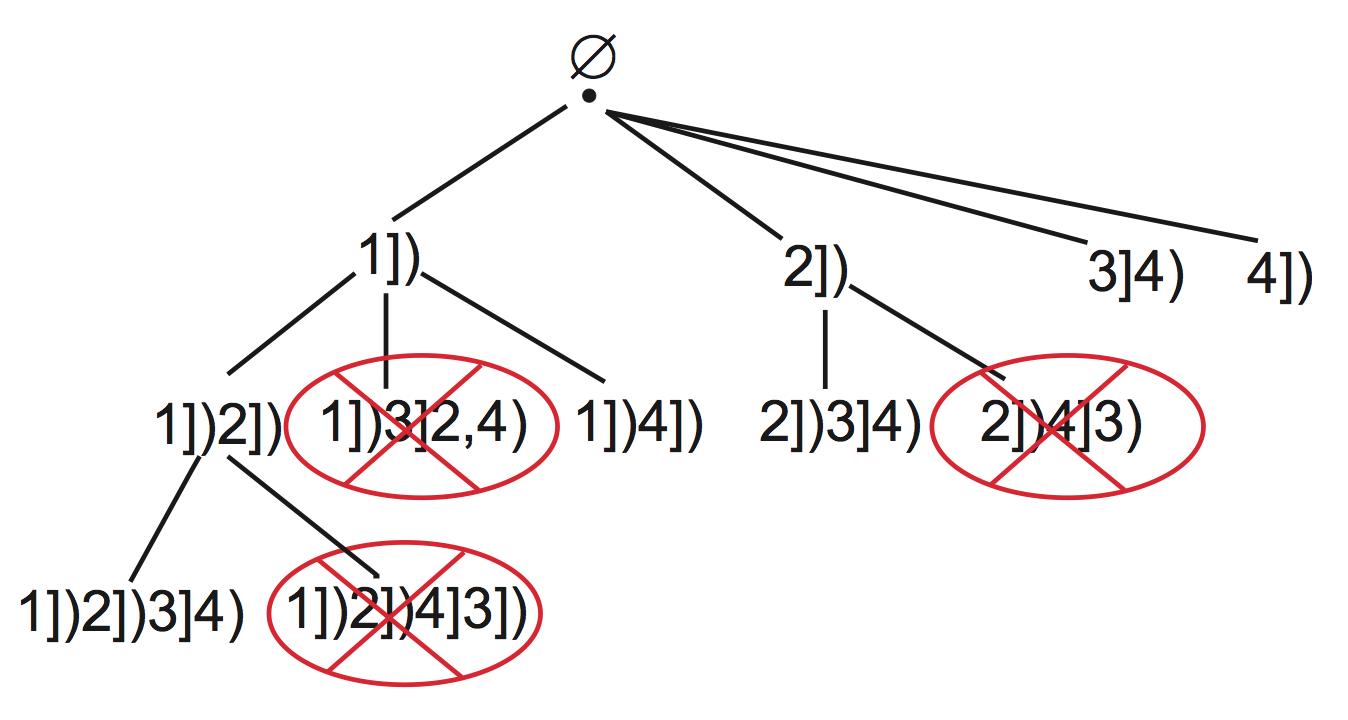
\includegraphics[width=0.5\textwidth]{cbo_tree.png}
    \label{fig:cbo_tree}
    \caption{Extent-based CbO recursion tree.}
\end{figure}

% section ordered_sets (end)

\section{\rus{Методы машинного обучения и майнинга данных}} % (fold)
\label{sec:mldm}

\noindent\textbf{Q:}\rus{Задача классификации.  Методы 1-Rule и ближайшего соседа
(kNN). Методы оценки качества. Скользящий контроль (crossvalidation). Точность и
полнота. ROC-кривые.}

\hfill\\\textbf{A:}

\hfill\\\textbf{Q:}\rus{Задача классификации.  Метод Naïve Bayes. Методы оценки
качества. Скользящий контроль (crossvalidation). Точность и полнота. ROC-кривые.}

\hfill\\\textbf{A:}

\hfill\\\textbf{Q:}\rus{Задача классификации. Деревья решений (на примере ID3 или
C4.5). Методы оценки качества. Скользящий контроль (crossvalidation). Точность и
полнота. ROC-кривые.}

\hfill\\\textbf{A:}

\hfill\\\textbf{Q:}\rus{Задача кластеризации. Метод k-средних. Метод K-медоидов.
Силуэт кластеризации (silhouette).}

\hfill\\\textbf{A:}

\hfill\\\textbf{Q:}\rus{Задача кластеризации. Иерархическая кластеризация. Подходы
AGNES (AGglomerative NESting) и DIANA (DIvisive ANAlysis).}

\hfill\\\textbf{A:}

\hfill\\\textbf{Q:}\rus{Поиск ассоциативных правил и частых множеств признаков.
Алгоритм Apriori. Меры качества правил (support и confidence).}

\hfill\\\textbf{A:}
See a similar question in sec.\ref{sec:ordered_sets}.

\hfill\\\textbf{Q:}\rus{Рекомендательные системы. Алгоритмы рекомендаций на основе
сходства по пользователям и на основе сходства по признакам. Меры сходства. Меры
качества рекомендаций: средняя абсолютная ошибка (MAE), точность и полнота.}

\hfill\\\textbf{A:}

\hfill\\\textbf{Q:}\rus{Кластеризация на графах. Спектральная кластеризация. Спектральная
кластеризация двудольного графа и бикластеризация (на примере объектно-признаковой
бикластеризации).}

\hfill\\\textbf{A:}

\hfill\\\textbf{Q:}\rus{Предмет и задачи машинного обучения и разработки (майнинга)
данных. Таксономия методов. Примеры задач.}

\hfill\\\textbf{A:}

% section mldm (end)

\end{document}
